%%%%%%%%%%%%%%%%%%%%%%%%%%%%%%%%%%%%%%%%%%%%%%%%%%%%%%%%%%%%
%%%%%%%%%%%%%%%%%%%%%%%%%%%%%%%%%%%%%%%%%%%%%%%%%%%%%%%%%%%%
%%%%%%%%%%%%%%%%%%%%%%%%%%%%%%%%%%%%%%%%%%%%%%%%%%%%%%%%%%%%
\section{Discrete Operators in  \texttt{dune-pdelab}}
%%%%%%%%%%%%%%%%%%%%%%%%%%%%%%%%%%%%%%%%%%%%%%%%%%%%%%%%%%%%
%%%%%%%%%%%%%%%%%%%%%%%%%%%%%%%%%%%%%%%%%%%%%%%%%%%%%%%%%%%%
%%%%%%%%%%%%%%%%%%%%%%%%%%%%%%%%%%%%%%%%%%%%%%%%%%%%%%%%%%%%

\subsection{Conforming Finite Elements for the Dirichlet Problem}

\begin{frame}
\frametitle<presentation>{Residual Formulation Revisited}
Recall the unconstrained problem in weighted residual form:
\begin{equation*}
u_h\in U_h\ : \qquad r_h(u_h,v) = 0 \qquad \forall
v\in V_h .
\end{equation*}

Solving it in the original basis
reduces to the solution of a nonlinear algebraic problem:
\begin{equation*}
\begin{split}
\mathbf{u}\in\mathbf{U} : \qquad
& r_h\left(\text{FE}_{\Phi_{U_h}}(\mathbf{u}),\psi_i\right) = 0, \quad
i\in\mathcal{I}_{V_h} \\
\Leftrightarrow \  & \mathcal{R}(\mathbf{u}) = \mathbf{0}
\end{split}
\end{equation*}
where we introduced the nonlinear residual map $\mathcal{R} :
\mathbf{U} = \mathbb{K}^{\mathcal{I}_{V_h}} \to \mathbb{K}^{\mathcal{I}_{V_h}}$ which is defined as 
\begin{equation*}
\left(
\mathcal{R}(\mathbf{u})\right)_i =
r_h(\text{FE}_{U_h}(\mathbf{u}),\psi_i).
\end{equation*}
$\Phi_{V_h} = \{\psi_i\,|\, i\in\mathcal{I}_{V_h}\}$ is the basis of $V_h$.  
\end{frame}

\begin{frame}
\frametitle<presentation>{Evaluation of Residual Map}
Using splitting and localization properties we obtain
\begin{align*}
\mathcal{R}(\mathbf{u}) 
&= \sum_{e\in E^0_h} \mathbf{R}_e^T\bm{\alpha}^\text{vol}_{h,e}(\mathbf{R}_e\mathbf{u}) 
&&+ \sum_{e\in E^0_h} \mathbf{R}_e^T\bm{\lambda}^\text{vol}_{h,e} \\
&+ \sum_{f\in E^1_h}
\mathbf{R}_{l(f),r(f)}^T\bm{\alpha}^\text{skel}_{h,f}(\mathbf{R}_{l(f),r(f)}\mathbf{u}) 
&&+ \sum_{f\in E^1_h} \mathbf{R}_{l(f),r(f)}^T\bm{\lambda}^\text{skel}_{h,f}\\
&+ \sum_{b\in B^1_h} \mathbf{R}_{l(b)}^T\bm{\alpha}^\text{bnd}_{h,b}(\mathbf{R}_{l(b)}\mathbf{u})
&&+ \sum_{b\in B^1_h} \mathbf{R}_{l(b)}^T\bm{\lambda}^\text{bnd}_{h,b}.
\end{align*}
Restriction and prolongation operators are generic from local to global map.
\end{frame}

The $\bm{\alpha}^\ast$ and $\bm{\lambda}^\ast$ terms are given below.

\begin{frame}<article>
\frametitle<presentation>{Local Residual Methods $\bm{\alpha}^\ast$ and $\bm{\lambda}^\ast$}
{\small\begin{align*}
\left(\bm{\alpha}^\text{vol}_{h,e}(\mathbf{R}_e\mathbf{u})\right)_i &=
\alpha^\text{vol}_{h,e}(\chi_e u_h,\chi_e \psi_{g(e,i)}), &
\left(\bm{\lambda}^\text{vol}_{h,e}\right)_i &=
\lambda^\text{vol}_{h,e}(\chi_e \psi_{g(e,i)}),
\end{align*}}
{\small
\begin{align*}
\left(\bm{\alpha}^\text{skel}_{h,f}(\mathbf{R}_{l(f),r(f)}\mathbf{u})\right)_i &=
\left\{\begin{array}{ll}
\alpha^\text{skel}_{h,f}(\chi_{l(f)\cup r(f)} u_h,\chi_{l(f)}\psi_{g(l(f),i)}) & 0\leq i<k(l(f))\\
\mbox{}\\
\alpha^\text{skel}_{h,f}(\chi_{l(f)\cup r(f)} u_h,\chi_{r(f)}\psi_{g(r(f),i')}) & 0\leq i'=i-k(l(f))<k(r(f))
\end{array}\right., \\
\left(\bm{\lambda}^\text{skel}_{h,f}\right)_i &=
\left\{\begin{array}{ll}
\lambda^\text{skel}_{h,f}(\chi_{l(f)}\psi_{g(l(f),i)}) & 0\leq i<k(l(f))\\
\mbox{}\\
\lambda^\text{skel}_{h,f}(\chi_{r(f)}\psi_{g(l(r),i')}) & 0\leq i'=i-k(l(f))<k(r(f))
\end{array}\right.
\end{align*}}
{\small\begin{align*}
\left(\bm{\alpha}^\text{bnd}_{h,b}(\mathbf{R}_{l(b)}\mathbf{u})\right)_i &=
\alpha^\text{bnd}_{h,b}(\chi_{l(b)} u_h,\chi_{l(b)} \psi_{g(l(b),i)}), &
\left(\bm{\lambda}^\text{bnd}_{h,e}\right)_i &=
\lambda^\text{bnd}_{h,b}(\chi_{l(b)}\psi_{g(l(b),i)}).
\end{align*}}
At most six element-local methods for $\bm{\alpha}^\text{vol}_{h,e}$,
$\bm{\alpha}^\text{skel}_{h,f}$, $\bm{\alpha}^\text{bnd}_{h,b}$,
$\bm{\lambda}^\text{vol}_{h,e}$, $\bm{\lambda}^\text{skel}_{h,f}$ and
$\bm{\lambda}^\text{bnd}_{h,b}$ need to be implemented by the user.
\end{frame}

Now we apply this to the Dirichlet problem of the Laplace equation.

\begin{frame}
\frametitle<presentation>{Conforming Method for the Dirichlet Problem}
Consider
\begin{subequations}
\begin{align*}
                -\Delta u &= 0& \text{in }& \Omega\subseteq\mathbb{R}^n,\\
                        u &= g& \text{on }& \Gamma_D\subseteq\partial\Omega.\\
\end{align*}
\end{subequations}
The discrete problem reads as follows.
\begin{equation*}
u_h\in w_h+\tilde{U}_h^k : \quad \int_\Omega \nabla u_h \cdot 
\nabla v \diffd x = 0 \qquad \forall v\in \tilde{U}^k_h.
\end{equation*}

Here, $r_h$ contains just the $\bm{\alpha}^\text{vol}_{h,e}$ volume term:
\begin{equation*}
r_h(u,v) = \int_\Omega \nabla u_h\cdot\nabla v \diffd x = \sum_{e\in
E_h^0} \int_{\Omega_e} \nabla u_h\cdot\nabla v \diffd x.  
\end{equation*}

The element integral is evaluated as in the integration example above.
\end{frame}

\begin{frame}
\frametitle<presentation>{Local Residual Evaluation Class}
To implement a discretization one has to implement a class providing
methods for evaluation of $\bm{\alpha}^\text{vol}_{h,e}$,
$\bm{\alpha}^\text{skel}_{h,f}$, $\bm{\alpha}^\text{bnd}_{h,b}$,
$\bm{\lambda}^\text{vol}_{h,e}$, $\bm{\lambda}^\text{skel}_{h,f}$ and
$\bm{\lambda}^\text{bnd}_{h,b}$.

The following listing contains the $\bm{\alpha}^\text{vol}_{h,e}$ for
the Dirichlet problem of the Laplace equation.

Line \ref{laplace:JacApply} provides a generic implementation of
$\nabla \bm{\alpha}^\text{vol}_{h,e}(\mathbf{R}_e\mathbf{u}) \mathbf{R}_e\mathbf{u}$
through numerical differentiation.

Line \ref{laplace:Jac} provides a generic implementation of
$\nabla \bm{\alpha}^\text{vol}_{h,e}(\mathbf{R}_e\mathbf{u})$ through
numerical differentiation.

Line \ref{laplace:Pattern} provides a default implementation for the
sparsity pattern of the operator: All degrees of freedom of an element
depend on each other.

Lines \ref{laplace:FirstFlag}---\ref{laplace:LastFlag} tell the
generic assembler which methods are provided in this class.

Main work is done starting in line \ref{laplace:AlphaVolume} with
method \lstinline{alpha_volume}.
\end{frame}

\begin{frame}<presentation>[fragile,allowframebreaks,allowdisplaybreaks]
\frametitle<presentation>{Dirichlet Problem Listing}
\framesubtitle<presentation>{File \texttt{examples/laplacedirichletop.hh}}
\lstinputlisting[basicstyle=\ttfamily\scriptsize,numbers=left, 
numberstyle=\tiny, numbersep=5pt]{../../examples/laplacedirichletop.hh}
\end{frame}
\mode<article>{
\begin{Lst}[File examples/laplacedirichletop.hh] \mbox
\nopagebreak
\lstinputlisting[basicstyle=\ttfamily\scriptsize,numbers=left, 
numberstyle=\tiny, numbersep=5pt]{../../examples/laplacedirichletop.hh}
\end{Lst}}

\begin{frame}
\frametitle<presentation>{Dirichlet Driver}
The following listing now solves the problem for a given mesh and
finite element space.

Lines \ref{lapdriver:FirstKnown}---\ref{lapdriver:LastKnown} set up
the grid function space, assemble constraints and initialize a
coefficient vector as it has been shown before.

New in line \ref{lapdriver:ISTLBackend} is the provision of the ISTL
backend in order to make the coefficient vector an ISTL vector.

Line \ref{lapdriver:ResEval} instantiates a local residual evaluation
object.

\lstinline{Dune::PDELab::GridOperatorSpace} in
line \ref{lapdriver:GOS} is the generic assembler which provides the
following methods:
\begin{itemize}
\item \lstinline{residual()} to evaluate the global residual
$\mathcal{R}(\mathbf{u})$.
\item \lstinline{jacobian()} to assemble the Jacobian matrix
$\nabla\mathcal{R}(\mathbf{u})$. 
\item \lstinline{jacobian_apply()} to compute Jacobian times vector
$\nabla\mathcal{R}(\mathbf{u})\mathbf{u}$. 
\end{itemize} 
The transformations due to constraints are not implemented yet, except
Dirichlet constraints.
\end{frame}

\begin{frame}
\frametitle<presentation>{Dirichlet Driver (Contd.)}
Now we go about to setup and solve the linear system in two ways:
(1) with setting up a matrix and (2) \textit{without} setting up a
matrix. 

Line \ref{lapdriver:MatrixType} extracts the matrix type from the
operator space, which is an ISTL matrix here.

Line \ref{lapdriver:MatrixSetup} instantiates a sparse matrix, where
the sparsity pattern is determined by the local operator.

In line \ref{lapdriver:JacoAssemble} the Jacobian is assembled (at the
initial solution).

Lines \ref{lapdriver:ISTLFirst}---\ref{lapdriver:ISTLLast} set up ISTL
solver components: An operator used by CG, an SSOR preconditioner, a
CG solver and a status variable.

Following Algorithm \ref{algo:ConstrainedNewton} specialized for a
linear system, we 
\begin{itemize}
\item compute the residual in line \ref{lapdriver:Residual},
\item solve the update equation in line \ref{lapdriver:UpdateEq}
\item and do the update in line \ref{lapdriver:Update}.
\end{itemize}
\end{frame}

\begin{frame}
\frametitle<presentation>{Dirichlet Driver (Contd.)}
Alternatively, we now show how to solve the system in a matrix-free
variant. 

In line \ref{lapdriver:OnTheFlyOp} we set up an operator for the CG
method that uses \lstinline{jacobian_apply} of the grid operator space
to do the matrix vector product.

Since we do not have an assembled Jacobian only simple preconditioners
can be used. We use Richardson (= no preconditioning) in
line \ref{lapdriver:Richardson}. 

The new CG solver is setup in line \ref{lapdriver:NewCG} and used in
lines \ref{lapdriver:AltSolverFirst}---\ref{lapdriver:AltSolverLast}
as before.

Finally, lines \ref{lapdriver:VTKFirst}---\ref{lapdriver:VTKLast}
provide VTK output.
\end{frame}

\begin{frame}<presentation>[fragile,allowframebreaks,allowdisplaybreaks]
\frametitle<presentation>{Dirichlet Driver Listing}
\framesubtitle<presentation>{File \texttt{examples/laplacedirichlet.hh}}
\lstinputlisting[basicstyle=\ttfamily\scriptsize,numbers=left, 
numberstyle=\tiny, numbersep=5pt]{../../examples/laplacedirichlet.hh}
\end{frame}
\mode<article>{
\begin{Lst}[File examples/laplacedirichlet.hh] \mbox
\nopagebreak
\lstinputlisting[basicstyle=\ttfamily\scriptsize,numbers=left, 
numberstyle=\tiny, numbersep=5pt]{../../examples/laplacedirichlet.hh}
\end{Lst}}

\begin{frame}<presentation>
\frametitle<presentation>{Dirichlet Problem Solution}
The Laplace example can now be run with all conforming spaces (and
also nonconforming ones like the rotated bilinear) and in any space
dimension.

Here is the Result for $Q_1$ in $2d$ and $3d$:
\begin{center}
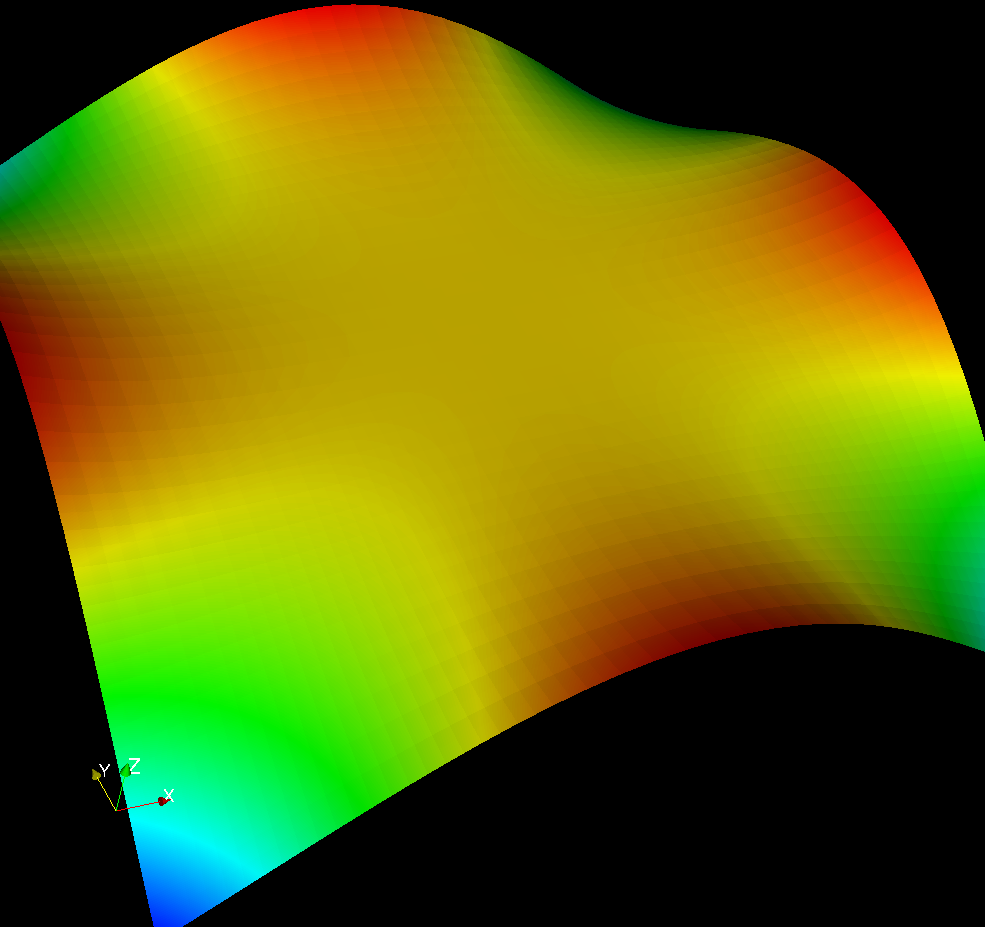
\includegraphics[width=0.49\textwidth]{./EPS/q1laplace}\hfill
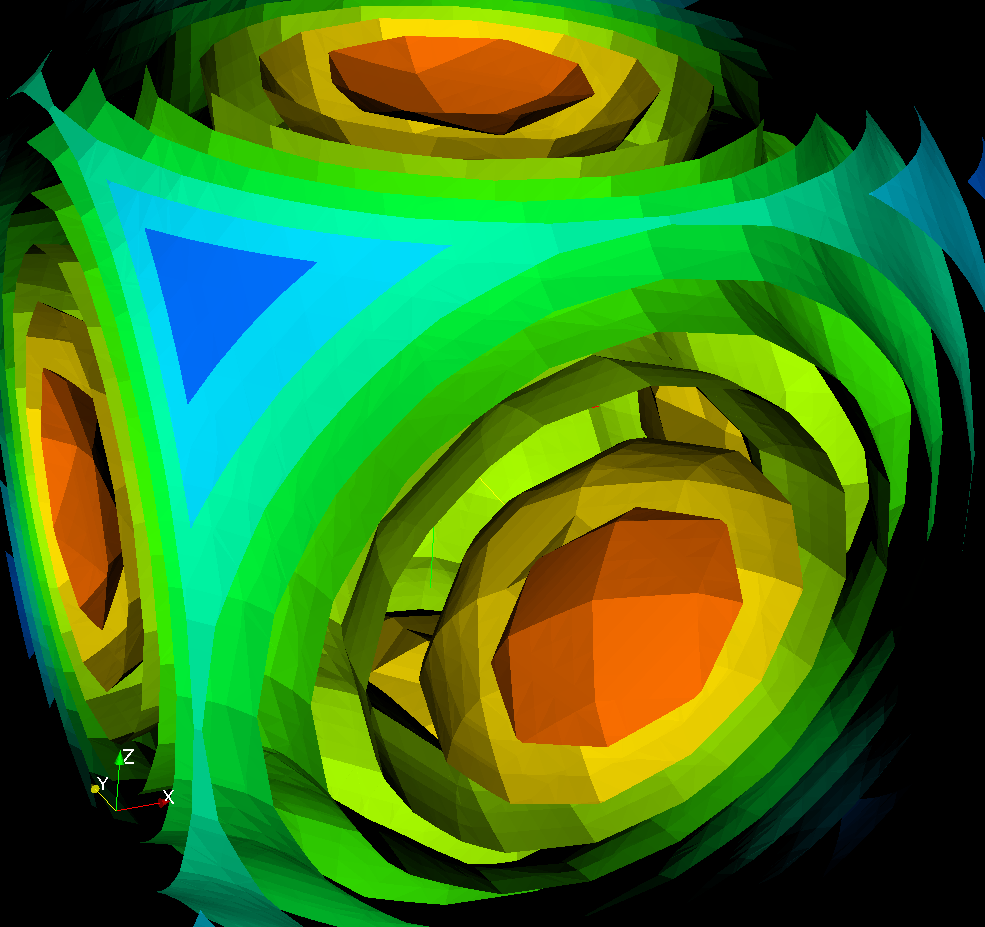
\includegraphics[width=0.49\textwidth]{./EPS/q1laplace3d}
\end{center}
\end{frame}

Figure \ref{fig:LaplaceResult} shows the output of the Laplace example
for $Q_1$ in $2d$ and $3d$. 

\mode<article>{
\begin{figure}
\begin{center}
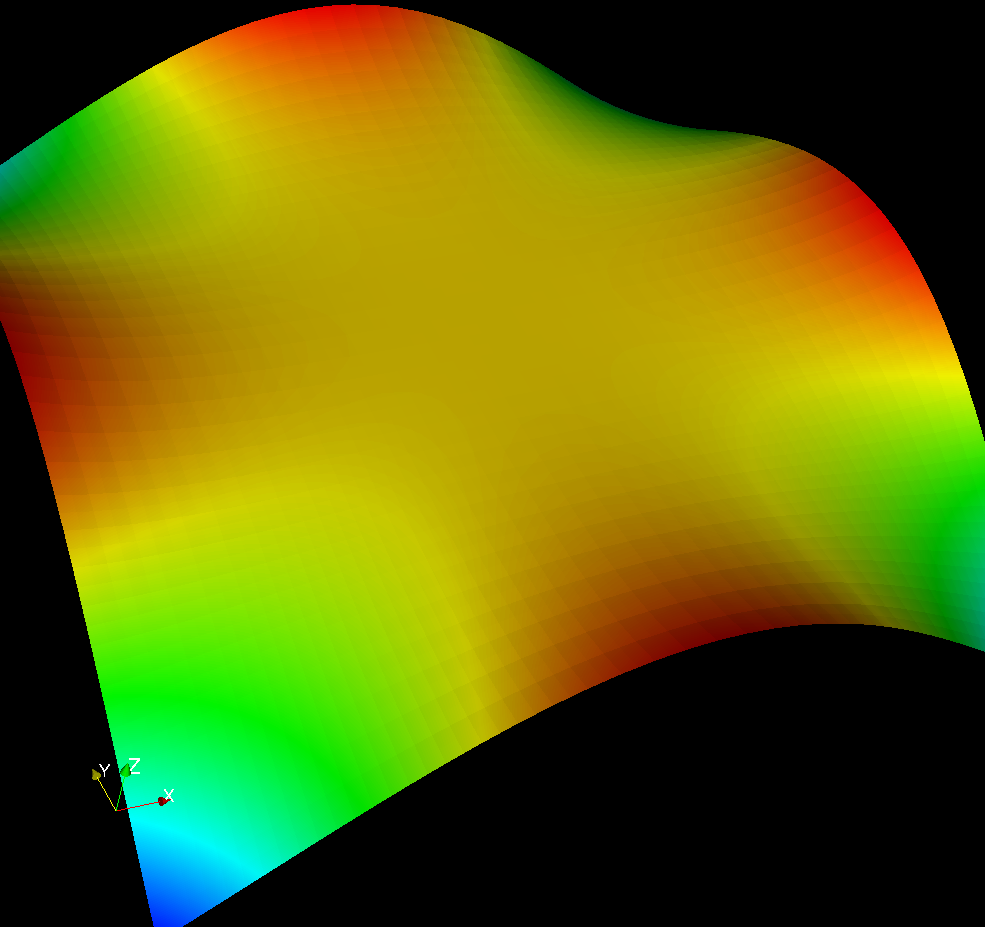
\includegraphics[width=0.49\textwidth]{./EPS/q1laplace}\hfill
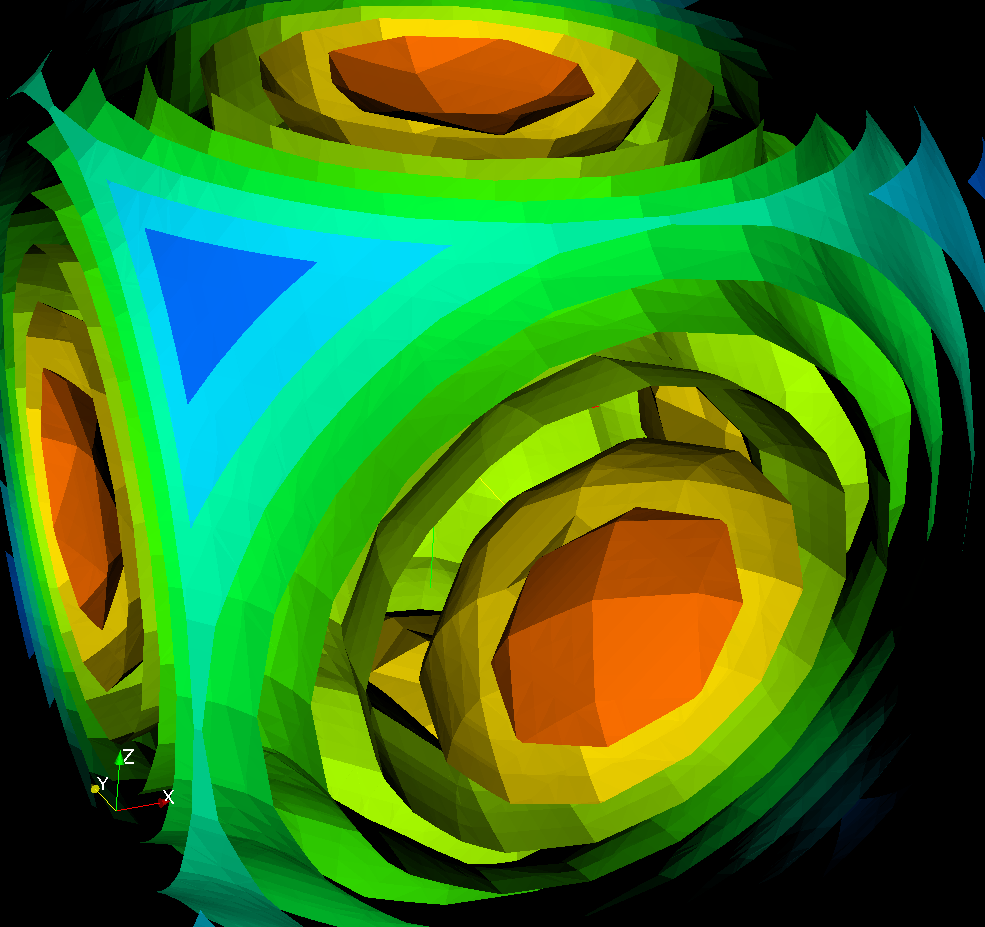
\includegraphics[width=0.49\textwidth]{./EPS/q1laplace3d}
\end{center}
\caption{Visualization of the Laplace example in $2d$ and $3d$.}
\label{fig:LaplaceResult}
\end{figure}
}

Here are some code metrix to show how much work it is to implement
various components.

\begin{frame}
\frametitle<presentation>{Some Code Metrics}
\begin{itemize}
\item Function spaces
\begin{itemize}
\item $Q_1$, $d=2$ : 80 lines + 20 lines for Dirichlet constraints.
\item $P_k$, $d=2$, $k$ a template parameter : 358 lines.
\item RT$_0$, $d=2$ : 187 lines.
\end{itemize}
\item Operators
\begin{itemize}
\item Laplace equation, Dirichlet b.c., conforming (any $d$, any $p$) : 79 lines.
\item Laplace equation, Dirichlet b.c., cell-centered FV (any $d$) : 138 lines.
\item Poisson equation, Dirichlet and Neumann b.c., conforming (any $d$, any $p$) : 196 lines.
\item Poisson equation, Dirichlet and Neumann b.c., $H(\text{div})$
conforming (mixed) method (any $d$, any $p$) : 267 lines. 
\end{itemize}
\end{itemize}
\end{frame}

And finally some computation times for various methods.

\begin{frame}
\frametitle<presentation>{Masters of the Unit Square}
Solve $-\Delta u = 0$ in $\Omega=(0,1)^2$, $u=g$ on $\partial\Omega$, $\mathcal{I}_{U_h}=10^6$, time in $s$.

\vspace{-4mm}
\begin{center} \small
\begin{tabular}{|l||r|r|r|r|}
\hline
Grid & GFS setup & Matrix setup & $\nabla\mathcal{R}$ eval. & $\mathcal{R}$ eval.\\
\hline
\multicolumn{5}{|c|}{Bilinear ($Q_1$) finite elements}\\
\hline
YaspGrid & 0.38 & 4.1 & 6.6 & 1.9 \\
UGGrid   & 0.94 & 4.8 & 9.0 & 2.5 \\
\hline
\multicolumn{5}{|c|}{Cell-centered finite volumes}\\
\hline
YaspGrid & 0.23 & 3.7 & 4.6 & 2.5 \\
UGGrid   & 0.58 & 5.2 &13.3 & 6.8 \\
\hline
\multicolumn{5}{|c|}{Linear ($P_1$) finite elements}\\
\hline
UGGrid      & 1.42 & 5.7 & 7.2 & 2.6 \\
AlbertaGrid & 1.90 & 6.2 & 6.1 & 3.0 \\
ALUGrid     & 1.78 & 6.0 & 6.0 & 2.8 \\
\hline
\multicolumn{5}{|c|}{Quartic ($P_4$) finite elements}\\
\hline
UGGrid      & 0.33 & 9.3 & 73.1 & 5.1 \\
AlbertaGrid & 0.34 & 9.3 & 77.6 & 4.9 \\
ALUGrid     & 0.31 & 9.0 & 72.0 & 4.9 \\
\hline
\end{tabular}
\end{center}

\end{frame}


\subsection{Summary}

\begin{frame}
\frametitle<presentation>{Operator Summary}
In order to implement a discretization in PDELab You have to do the
following:
\begin{itemize}
\item Write your problem in residual based form and decide which
integrals contribute to each of the volume, skeleton and boundary
terms.
\item Implement a local residual class containing:
\begin{itemize}
\item Sparsity pattern definition methods for volume/skeleton (default
versions provided, only required if matrix is assembled).
\item Residual evaluation for volume/skeleton/boundary contributions.
\item Jacobian evaluation (default with numerical differentiation
provided).
\item Jacobian application (default with numerical differentiation
provided).
\item Jacobians must be implemented, if numerical evaluation is not
desired or approximations (``Picard'') are required.
\item In the linear case, implementation of Jacobian (``local stiffness
matrix'') and default implementation of residual evaluation is more
efficient. 
\end{itemize}
\item Put everything into a grid operator space.
\end{itemize}
\end{frame}

\begin{frame}
\frametitle<presentation>{Final Notes}
Things that are still to do:
\begin{itemize}
\item Implementation of constraints (only Dirichlet is done so far,
the transformation matrices can be assembled but not applied). 
\item Newton and time-stepping schemes.
\item Real applications.
\end{itemize}

\medskip
\begin{center}
\textbf{Acknowledgements}

BMBF Project AdaptHydroMod Förderkennzeichen 03BAPAF2

StatoilHydro Research
\end{center}
\end{frame}

\cleardoublepage
